\chapter{Implementation}

The FFT application has been implemented in C/C++, CUDA, OpenCL, DirectCompute and OpenGL on a GeForce GTX 670 and Radeon R7 260X graphics card and a Core i7 3770K 3.5GHz CPU.

\section{Benchmark application GPU}

\subsection{FFT}

\subsubsection{Setup}

The implementation of the FFT algorithm on a GPU can be broken down into a few steps, see figure \ref{fig:algorithm-overview} for a simplified overview. The application setup differs among the tested technologies, however some steps can be generalized; get platform and device information, allocate device buffers and upload data to device.
\begin{figure}[H]
	\centering
	\includestandalone[width=\textwidth]{figures/overview}
	\caption{Overview of the events in the algorithm.}
	\label{fig:algorithm-overview}
\end{figure}

The next step is to calculate the specific FFT arguments for a $N$-point sequence for each kernel. The most important difference between devices and platforms are local memory capacity and thread and block configuration. Threads per block was selected for the best performance. See table \ref{tab:threads-per-block} for details.
\begin{table}
	\centering
	\includestandalone[width=\textwidth]{tables/threadsperblock}
	\caption{Shared memory size in bytes, threads and block configuration per device.}
	\label{tab:threads-per-block}
\end{table}

\subsubsection{Butterfly}

The implementation of a $N$-point radix-2 FFT algorithm have $\log_2 N$ stages with $N/2$ butterfly operations per stage. A butterfly operation is an addition, a subtraction, followed by a multiplication by a twiddle factor, see figure \ref{fig:butterfly}.
\begin{figure}[H]
	\centering
	% FFT Butterfly
\tikzstyle{n}= [circle, fill, minimum size=4pt,inner sep=0pt, outer sep=0pt]
\tikzstyle{mul} = [circle,draw,inner sep=-1pt, minimum size=7pt]
\tikzstyle{sub} = [circle,draw,inner sep=-1pt, minimum size=7pt]
\tikzstyle{add} = [circle,draw,inner sep=-1pt, minimum size=7pt]

\begin{tikzpicture}[
	yscale=1.3,
	xscale=1.8,
	node distance=0.7cm,
	auto]
    
	\node[n, pin={[pin edge={latex'-,black}]left:$x(0)$}] (N-0-0) at (0,-0) {};
	\node[n, pin={[pin edge={latex'-,black}]left:$x(1)$}] (N-0-1) at (0,-1) {};
                            
	\node[add, name=N-1-0, pin={[pin edge={-latex',black},pin distance=1.175cm]right:$X(0)$}] at (1,-0) {${+}$};
	\node[sub, name=N-1-1, label={[label distance=-10pt]90:${-}$}] at (1,-1) {};
            
	\node[mul, right of=N-1-1, label={above right:\tiny $W^{k}_{N}$},
		pin={[pin edge={-latex',black}]right:$X(1)$}] (N-2-1) {${\times}$};       

	\path (N-0-0) edge[-latex'] (N-1-0);	
	\path (N-0-1) edge[-latex'] (N-1-1);
	\path (N-1-1) edge[-latex'] (N-2-1);
      
    % Connect nodes
    \foreach \src / \dst in {	0/0, 0/1, 1/0, 1/1}
       \path (N-0-\src.east) edge[-latex'] (N-1-\dst.west);
       
\end{tikzpicture}
	\caption{Butterfly operations}
	\label{fig:butterfly}
\end{figure}

\subsubsection{Thread and block scheme}

The threading scheme was one butterfly per thread, so that a sequence of sixteen points require eight threads. Each platform was configured to a number of threads per block (see table \ref{tab:threads-per-block}) and any sequences requiring more butterfly operations then the threads per block configuration needed the computations to be split over several blocks. In the case of sequence exceeding one block, the sequence is mapped over the \texttt{blockIdx.y} dimension with size \texttt{gridDim.y}. The block dimension \texttt{blockIdx.x} is used to calculate sequence id when running a batch of sequences, the block dimensions are limited to $2^{31}$, $2^{16}$, $2^{16}$ respectively for \texttt{x}, \texttt{y}, \texttt{z}. Example: if the threads per block limit is two, then four blocks would be needed for a sixteen point sequence.

\begin{figure}[htbp]
	% FFT Butterfly
\tikzstyle{n}= [circle, fill, minimum size=4pt,inner sep=0pt, outer sep=0pt]
\tikzstyle{mul} = [circle,draw,inner sep=-1pt]

% Define two helper counters
\newcounter{x}\newcounter{y}
\begin{tikzpicture}[%
	yscale=0.6,
	xscale=1.15,
	node distance=0.25cm,
	auto]
    % The strategy is to create nodes with names: N-column-row
    % Input nodes are named N-0-0 ... N-0-15
    % Output nodes are named N-10-0 ... N-10-15

    % Draw inputs
    \foreach \y in {0,...,15}
        \node[n, pin={[pin edge={latex'-,black}]left:$x(\y)$}] (N-0-\y) at (0,-\y) {};
              
    % Draw outputs
    \foreach \y in {0,...,15}
        \node[n, pin={[pin edge={-latex',black}]right:$X(\y)$}] (N-11-\y) at (8,-\y) {};
              
   % draw connector nodes
    \foreach \y in {0,...,15}
        \foreach \x / \c in {1/1,2/3,3/4,4/6,5/7,6/9,7/10}
            \node[n, name=N-\c-\y] at (\x,-\y) {};
            
    % draw x nodes
    \foreach \y in {0,...,7}
        \foreach \x / \c  in {1/2}
            \node[mul, right of=N-\x-\y] (N-\c-\y) {};            
    \foreach \y in {8,...,15}
        \foreach \x / \c  in {1/2}
            \node[mul, right of=N-\x-\y] (N-\c-\y) {${\times}$};
    % 
    \foreach \y in {0,...,3}
        \foreach \x / \c  in {4/5}
            \node[mul, right of=N-\x-\y] (N-\c-\y) {};
    \foreach \y in {4,...,7}
        \foreach \x / \c  in {4/5}
            \node[mul, right of=N-\x-\y] (N-\c-\y) {${\times}$};
    \foreach \y in {8,...,11}
        \foreach \x / \c  in {4/5}
            \node[mul, right of=N-\x-\y] (N-\c-\y) {};
    \foreach \y in {12,...,15}
        \foreach \x / \c  in {4/5}
            \node[mul, right of=N-\x-\y] (N-\c-\y) {${\times}$};
    % 
    \foreach \y in {0,2,4,6,8,10,12,14}
        \foreach \x / \c  in {7/8}
            \node[mul, right of=N-\x-\y] (N-\c-\y) {};
    \foreach \y in {1,3,5,7,9,11,13,15}
        \foreach \x / \c  in {7/8}
            \node[mul, right of=N-\x-\y] (N-\c-\y) {${\times}$};    

    % horizontal connections
    % Note the use of simple counter arithmetics to get correct
    % indexes.
    \foreach \y in {0,...,15}
    {
		\foreach \x in {0,1,3,4,7}
		{
			\setcounter{x}{\x}\stepcounter{x}
			\path (N-\x-\y) edge[-] (N-\arabic{x}-\y);
		}
	}
       
    % Draw the W_16 coefficients
    \setcounter{y}{0}
    \foreach \i in {0,...,7}
    {
	   	\path (N-2-\arabic{y}) edge[-] node {} (N-3-\arabic{y});
	    \stepcounter{y}
    }
    \foreach \i in {0,...,7}
    {
    	\path (N-2-\arabic{y}) edge[-] node {\tiny $W^{\i}_{16}$} (N-3-\arabic{y});
        \stepcounter{y}
    }
    
    % Draw the W_8 coefficients
    \setcounter{y}{0}
    \foreach \tmp in {0,1}
	{
    	\foreach \i in {0,...,3}
    	{
        	\path (N-5-\arabic{y}) edge[-] node {} (N-6-\arabic{y});
        	\addtocounter{y}{1}
    	}
    	\foreach \i in {0,...,3}
    	{
        	\path (N-5-\arabic{y}) edge[-] node {\tiny $W^{\i}_{8}$} (N-6-\arabic{y});
        	\addtocounter{y}{1}
    	}
    }

    % Draw the W_4 coefficients
    \setcounter{y}{0}
	\foreach \tmp in {0,...,3}
	{    
		\foreach \i in {0,1}
		{
			\path (N-8-\arabic{y}) edge[-] node {} (N-9-\arabic{y});
			\stepcounter{y}
			\path (N-8-\arabic{y}) edge[-] node {\tiny $W^{\i}_{4}$} (N-9-\arabic{y});
			\stepcounter{y}
		}
    }
    
    % Connect nodes
    \foreach \sourcey / \desty in {	0/8,	1/9,	2/10,	3/11,
									4/12,	5/13,	6/14,	7/15,
									8/0,	9/1,	10/2,	11/3,
									12/4,	13/5,	14/6,	15/7}
       \path (N-0-\sourcey.east) edge[-] (N-1-\desty.west);
    \foreach \sourcey / \desty in {	0/4,	1/5,	2/6,	3/7,
									4/0,	5/1,	6/2,	7/3,
									8/12,	9/13,	10/14,	11/15,
									12/8,	13/9,	14/10,	15/11}
        \path (N-3-\sourcey.east) edge[-] (N-4-\desty.west);
    \foreach \sourcey / \desty in {	0/0,	1/2,	2/0,	3/2,
    								0/1,	1/3,	2/1,	3/3,
                                   	4/4,	5/6,	6/4,	7/6,
                                   	4/5,	5/7,	6/5,	7/7,
                                   	8/8,	9/10,	10/8,	11/10,
									8/9,	9/11,	10/9,	11/11,
									12/12,	13/14,	14/12,	15/14,
									12/13,	13/15,	14/13,	15/15}
	{
        \path (N-6-\sourcey.east) edge[-] (N-7-\desty.west);
        \path (N-9-\sourcey.east) edge[-] (N-10-\desty.west);
    }
    % Nodes are in bit-reverse order
    \foreach \sourcey / \desty in {	0/0,1/8,2/4,3/12,4/2,5/10,6,7/14,8/1,9,10/5,11/13,12/3,13/11,14/7,15/15}
	{
        \path (N-10-\sourcey.east) edge[-] (N-11-\desty.west);
    }
    
    % Add region boxes
	% Partial stage
	\def \lastNode {10}
	\node[draw,dashed,fit=(N-6-0) (N-\lastNode-3)] {};
	\node[draw,dashed,fit=(N-6-4) (N-\lastNode-7)] {};
	\node[draw,dashed,fit=(N-6-8) (N-\lastNode-11)] {};
	\node[draw,dashed,fit=(N-6-12) (N-\lastNode-15)] {};	
    % Complete stage
	\node[draw,densely dotted,fit=(N-0-0) (N-2-15),label=above:{stage 1}] {};
	\node[draw,densely dotted,fit=(N-3-0) (N-5-15),label=above:{stage 2}] {};
	\node[draw,fit=(N-6-0) (N-8-15),opacity=0,label=above:{stage 3},name=Stage-3] {};
	\node[draw,fit=(N-9-0) (N-\lastNode-15),opacity=0,label=above:{stage 4},name=Stage-4] {};
	\node[draw,fit=(N-11-0) (N-11-15),opacity=0,label=above:{output}] {};
	\node[draw,densely dotted,fit=(Stage-3) (Stage-4)] {};
	\node[draw,fit=(N-\lastNode-0) (N-11-15)] {};
\end{tikzpicture}
	\caption{Example flow graph of a sixteen-point FFT using (stage 1 and 2) Cooley-Tukey algorithm and (stage 3 and 4) constant geometry algorithm. The solid box is the bit-reverse order output. Dotted boxes are separate kernel launches, dashed boxes are data transfered to local memory before computing the remaining stages.}
	\label{fig:flowgraph-16}
\end{figure}

\subsubsection{Synchronization}

Thread synchronization is only available within a block. When the sequence or partial sequence fitted within a block all data was transferred to local memory before computing the last stages. If the sequence was larger and required more then one block the synchronization was handled by launching several kernels in the same stream to be executed in sequence. The kernel launched for block wide synchronization is called the global kernel and the kernel for thread synchronization within a block is called the local kernel. The global kernel had an implementation of the Cooley-Tukey FFT algorithm and the local kernel had constant geometry (same indexing for every stage). The last stage outputs from shared memory in bit reversed order to the global memory. See figure \ref{fig:flowgraph-16} where the sequence length is 16 and the threads per block is set to two.

\subsubsection{Calculation}

The indexing for the global kernel was calculated from the thread id and block id (\texttt{threadIdx.x} and \texttt{blockIdx.x} in CUDA) as seen in figure \ref{fig:code-global-index}. Input and output is done on the same index.
\begin{figure}[htbp]
	\centering
	\lstset{language=C++}
	\begin{framed}
	\begin{lstlisting}
int tid     = blockIdx.x * blockDim.x + threadIdx.x,
    io_low  = tid + (tid & (0xFFFFFFFF << stages_left)),
    io_high = index1 + (N >> 1);
	\end{lstlisting}
	\end{framed}
	\caption{ CUDA example code showing index calculation for each stage in the global kernel, N is the total number of points. \texttt{io\_low} is the index of the first input in the butterfly operation and \texttt{io\_high} the index of the second.}
	\label{fig:code-global-index}
\end{figure}

Index calculation for the local kernel is done once for all stages, see figure \ref{fig:code-local-index}. These indexes are separate from the indexing in the global memory. The global memory offset depends on threads per block (\texttt{blockDim.x} in CUDA) and block id.
\begin{figure}[htbp]
	\centering
	\lstset{language=C++}
	\begin{framed}
	\begin{lstlisting}
int n_per_block = N / gridDim.x.
    in_low      = threadId.x.
    in_high     = threadId.x + (n_per_block >> 1).
    out_low     = threadId.x << 1.
    out_high    = out1 + 1;
	\end{lstlisting}
	\end{framed}
	\caption{ CUDA example code showing index calculation for points in shared memory for the CUDA local kernel. }
	\label{fig:code-local-index}
\end{figure}

The last operation after the last stage is to perform the bit-reverse indexing operation, this is done when writing from shared to global memory. The implementation of bit reversing is available as a intrinsic integer instruction, see table \ref{tab:bit-reverse-intrinsics}. If instruction is not available figure \ref{fig:code-bit-reverse} shows the code used. The bit reversed value had to be right shifted the number of zeroes leading the number in a 32-bit int. Example of the bit-reverse index operation: index 8 of a 16 point sequence is bit-reversed to 1, in binary its 1000 reversed to 0001. Index 8 of a 32 point sequence is bit-reversed to 2, corresponds to 01000 to 00010. Figure \ref{fig:flowgraph-16} show the complete bit-reverse operations of a 16-point sequence in the output step after the last stage.

\begin{table}[!htbp]
	\centering
	\includestandalone[width=\textwidth]{tables/bit-reverse-intrinsics}
	\caption{Integer intrinsic bit-reverse function for different technologies.}
	\label{tab:bit-reverse-intrinsics}
\end{table}

\begin{figure}[!htbp]
	\centering
	\lstset{language=C++}
	\begin{framed}
	\begin{lstlisting}
x = (((x & 0xaaaaaaaa) >> 1) | ((x & 0x55555555) << 1));
x = (((x & 0xcccccccc) >> 2) | ((x & 0x33333333) << 2));
x = (((x & 0xf0f0f0f0) >> 4) | ((x & 0x0f0f0f0f) << 4));
x = (((x & 0xff00ff00) >> 8) | ((x & 0x00ff00ff) << 8));
return((x >> 16) | (x << 16));
	\end{lstlisting}
	\end{framed}
	\caption{ Code returning a bit reversed unsigned integer where x is the input. Only 32-bit integer input and output. }
	\label{fig:code-bit-reverse}
\end{figure}

\subsection{FFT 2D}

\begin{figure}[htbp]
	\centering
	\subfloat[Original image\label{image-1:lena}]{
		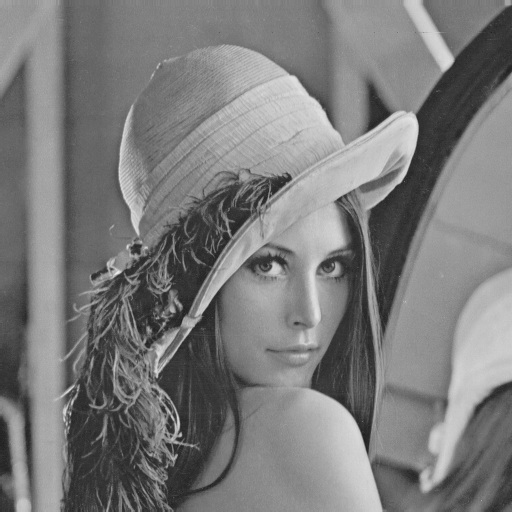
\includegraphics[keepaspectratio=true, scale=0.33]{images/lena.jpg}{}		
    }
    \hfill
    \subfloat[Magnitude representation\label{image-2:lena}]{
		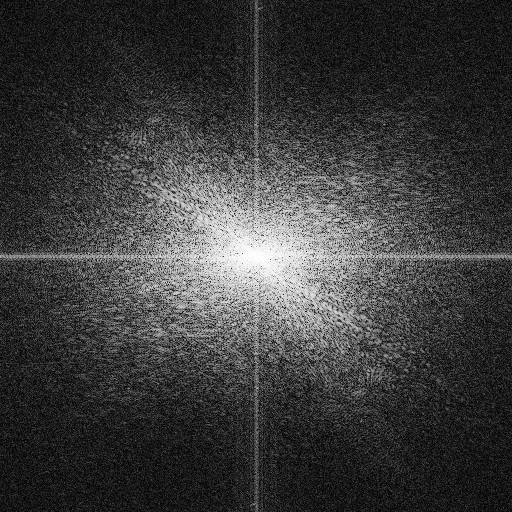
\includegraphics[keepaspectratio=true, scale=0.33]{images/lena_transformed.jpg}{}
    }
	\caption{Original image \ref{image-1:lena} transformed and represented with a quadrant shifted magnitude visualization (magnitude scale skewed for better visuals). \ref{image-2:lena}. }
    \label{fig:twodimentransform}
\end{figure}

The FFT algorithm for two dimensional data, such as images, is first transformed row wise (each row as a separate sequence) and then a transform of each column. The implementation performs a row wise transformation and then transposes the whole image twice, see figure \ref{lst:cuda:host-2d-example}. A transformed image is shown in figure \ref{fig:twodimentransform}.

\begin{figure}[htbp]
	\centering
	\begin{framed}
		\includestandalone[width=\textwidth]{code/cuda-host-2d}	
	\end{framed}
	\caption{CUDA host code for the 2D FFT algorithm.}
	\label{lst:cuda:host-2d-example}	
\end{figure}

The difference between the FFT kernel for 1D and 2D are the indexing scheme. 2D are indexed as rows at \texttt{blockIdx.x} and columns at $\texttt{threadIdx.x} + \texttt{blockIdx.y} \cdot \texttt{blockDim.x}$. For 2D \texttt{blockIdx.z} is used as the sequence id in a batch.

\subsubsection{Transpose}

The transpose kernel uses a different index mapping of the 2D-data and blocks/threads then the FFT kernel. The data is tiled in a grid pattern where each tile represents one block, indexed by \texttt{blockIdx.x} and \texttt{blockIdx.y}. The tile size is a multiple of 32 for both dimensions and limited to the size of the shared memory buffer, see table \ref{tab:threads-per-block} for specific size per technology. To avoid banking issues, the last dimension is increased with one but not used. However, resolving the banking issue have little effect on total running-time so when shared memory is limited to 32768, the extra column is not used. The tiles rows and columns are diveded over the \texttt{threadIdx.x} and \texttt{threadIdx.y} index respectively. See figure \ref{lst:cuda:device-transpose} for code example.

Shared memory example: The CUDA shared memory can allocate 49152 bytes and a single data point require $\texttt{sizeof(float)} \cdot 2 = 8$ bytes. That leaves room for a tile size of $64 \cdot (64 + 1) \cdot 8 = 33280$ bytes.

\begin{figure}[H]
	\centering
	\begin{framed}
		\includestandalone[width=\textwidth]{code/cuda-device-transpose}	
	\end{framed}
	\caption{CUDA device code for the transpose kernel.}
	\label{lst:cuda:device-transpose}	
\end{figure}

The transpose kernel uses the shared memory and tiling of the image to avoid large strides through global memory. Each block represents a tile in the image. The first step is to write the complete tile to shared memory and synchronize the threads before writing to the output buffer. Both reading from the input memory and writing to the output memory is performed in close stride. Figure \ref{fig:transpose-memory} shows how the transpose is performed in memory.

\begin{figure}[H]
	\centering
	\includestandalone[width=\textwidth]{figures/transpose-tile}
	\caption{Illustration of how shared memory is used in transposing an image. Input data is tiled and each tile is written to shared memory and transposed before written to the output memory. }
	\label{fig:transpose-memory}
\end{figure}

\subsection{Differences}

\subsubsection{Setup}

The major differences was mostly related to the setup phase. The CUDA implementation is the most straight forward, \texttt{cudaMalloc(...)} to allocate a buffer and \texttt{cudaMemcpy(...)} to populate it. With CUDA you can write the device code in the same file as the host code and even share functions, the OpenCL and OpenGL require a \texttt{char *} buffer and is most practical if written in seperate file and read as a file stream to a \texttt{char} buffer. DirectCompute Shaders are most easily compiled from file.

Figure \ref{fig:code:setup} demonstrates a simplified overview of how to setup the kernels in the different technologies.
\begin{figure}
	\centering
	\def \setupWidth {\textwidth / 2 - 20pt}	
	\subfloat[OpenCL setup\label{setup:cu}]{		
		\fbox{\includestandalone[width=\setupWidth]{code/setup/cu}}
	}	
	\hfill
	\subfloat[OpenCL setup\label{setup:ocl}]{		
		\fbox{\includestandalone[width=\setupWidth]{code/setup/ocl}}
	}
	\newline
	\subfloat[DirectCompute setup\label{setup:dx}]{		
		\fbox{\includestandalone[width=\setupWidth]{code/setup/dx}}
	}
	\hfill
	\subfloat[OpenGL setup\label{setup:gl}]{		
		\fbox{\includestandalone[width=\setupWidth]{code/setup/gl}}
	}
	\caption{A simplified overview of the different functions required for a kernel launch and upload of initial data. }		
	\label{fig:code:setup}
\end{figure}

\subsubsection{Kernel execution}

Kernel execution in CUDA is very much like any C-like language and the only difference is that the kernel launch syntax, $<<<$ and $>>>$, setting number of blocks and threads.

The other technologies require some more setup, OpenCL and OpenGL set one parameter per line. OpenCL maps with index whereas OpenGL maps with a string to the parameter. DirectCompute is best suited to use a constant buffer for the parameters, the constant buffer is read only and accessible globally over the kernel. DirectCompute and OpenGL share a similar launch style where the compute shader is set as the current program and then a dispatch call is made with the group (block) configuration. See table \ref{tab:kernel-execution} for a list of how the kernels are launched.

\begin{table}[H]
	\centering
	\includestandalone[width=\textwidth]{tables/kernel-execution}
	\caption{Table illustrating how to set parameters and launch a kernel.}
	\label{tab:kernel-execution}
\end{table}

\subsubsection{Kernel code}

This is the part where the code differ the least on but a few points. CUDA have the strongest support for a C/C++ -like language and only adds a function type specifier. The kernel program is accessible from the host via the \texttt{\_\_global\_\_} specifier. OpenCL share much of this but restricted to a C99-style in the current version (2.0). One difference is how one can reference global and local buffers, these must be specified with the specifier \texttt{\_\_global} or \texttt{\_\_local}.

DirectCompute and OpenGL Compute Shader uses HLSL (High-Level Shading Language) and GLSL (OpenGL Shading Language) respectively. These languages are similar and share the same restrictions compared to CUDA C/C++ and OpenCL C-code. Device functions can not use pointers or recursion. However these are of little importance for the performance since all code is in-lined in the compilation/building of the kernel program.

\subsubsection{Synchronization}

The synchronization of threads and blocks is slightly different, CUDA have the options to synchronize threads within a block and to synchronize host and device, the equivalent exists in all but DirectCompute (DirectX 11) where the device synchronization is not done trivially as with a blocking function call. See table \ref{tab:kernel-synchronization} for the code used for each technology.

\begin{table}[H]
	\centering
	\includestandalone[width=\textwidth]{tables/kernel-synchronization}
	\caption{Synchronize functions regarding within blocks/groups and between host and device. CUDA, OpenCL and DirectCompute uses the same kernel stream to run them sequentially; OpenGL uses the command \texttt{glMemoryBarrier(GL\_SHADER\_STORAGE\_BARRIER\_BIT)} to ensure kernels are run in the same order as launched.}
	\label{tab:kernel-synchronization}
\end{table}

\section{Benchmark application CPU}

\subsection{FFT with OpenMP}

The OpenMP implementation benefits in performance from calculating the twiddle factors in advance. The calculated values are stored in a buffer accessible from all threads. The next step is to calculate each stage of the FFT algorithm. Last is the output index calculation where elements are reordered. See figure \ref{fig:omp:overview} for an overview.

\begin{figure}
	\centering
	\includestandalone[width=\textwidth]{figures/omp-overview}
	\caption{OpenMP implementation overview transforming sequence of size $N$.}
	\label{fig:omp:overview}
\end{figure}

\subsubsection{Twiddle factors}

The twiddle factor are stored for each butterfly operation. To save time, only the real part are calculated and the imaginary part is retrieved from the real parts due to the fact that $\sin(x) = \cos(\pi/2 + x)$ and $\sin(\pi/2 + x) = -\cos(x)$ to store. See figure \ref{tab:omp:twiddle-overview} for an example. The calculations will be split among the threads by static scheduling in two steps, first calculate the real values, secondly copy from real to imaginary.

\begin{table}[H]
	\centering
	\begin{tabular}{|l|l|r|}
	\multicolumn{3}{c}{Table $W$} \\ \hline
	$i$ & $\Re(W)$ & $\Im(W)$ \\ \hline
	0 & $\cos(\alpha \cdot 0)$ & $\Re(W[4])$ \\
	1 & $\cos(\alpha \cdot 1)$ & $\Re(W[5])$ \\
	2 & $\cos(\alpha \cdot 2)$ & $\Re(W[6])$ \\
	3 & $\cos(\alpha \cdot 3)$ & $\Re(W[7])$ \\	
	4 & $\cos(\alpha \cdot 4)$ & $-\Re(W[0])$ \\
	5 & $\cos(\alpha \cdot 5)$ & $-\Re(W[1])$ \\
	6 & $\cos(\alpha \cdot 6)$ & $-\Re(W[2])$ \\
	7 & $\cos(\alpha \cdot 7)$ & $-\Re(W[3])$ \\ \hline
\end{tabular}
	\caption{Twiddle factors for a 16-point sequence where $\alpha = (2 \cdot \pi) / 16$. Each row $i$ corresponds to the $i$th butterfly operation.}
	\label{tab:omp:twiddle-overview}
\end{table}

\subsubsection{Butterfly}

The same butterfly operation uses the constant geometry index scheme. The indexes are not stored from one stage to the next but it makes the output come in continues order. The butterfly operations are split among the threads by static scheduling.

\subsubsection{Bit Reversed Order}

See figure \ref{fig:omp:bit-reverse-order} for code showing the bit reverse ordering operation in C/C++ code.

\begin{figure}[H]
	\centering
	\begin{framed}
		\includestandalone[width=\textwidth]{code/omp-bit-reverse}	
	\end{framed}
	\caption{ C/C++ code performing the bit reverse ordering of a N-point sequence. }
	\label{fig:omp:bit-reverse-order}
\end{figure}

\subsection{FFT 2D with OpenMP}

The implementation of 2D FFT with OpenMP run the transformations row wise and transposes the image and repeat. The twiddle factors are calculated once and stays the same.

\section{Benchmark configurations}

\subsection{Limitations}

All implementations are limited to handle sequences of $2^n$ length or $2^m \times 2^m$ where $n$ and $m$ are integers. The GPUs have a maximum of 2GB global memory available and the upper limit of 2D transformations are $m = 8192$ since the implementation uses two buffers and require $8192 \cdot 8192 \cdot \texttt{sizeof(float2)} \cdot 2 = 1073741824$ bytes, however the Radeon R7 260X card does not handle that size well and is limited to $m = 4096$ (and OpenGL is even limited to $m = 2048$).

\subsection{Testing}

All tests executed on the GPU utilize some implementation of event time stamps. The time stamp event retrieve the actual start of the kernel if the current stream is busy, if the time is measured by the host, some technologies are not able to synchronize and the timings may be very unstable. The CPU implementations used Windows \textit{QueryPerformanceCounter} function, which is a high resolution (<1{\micro}s) time stamp.

All tests on the GTX 670 are run in batches of constant size 1073741824 bytes. A batch with 256-point sequences would run a total of 262144 sequences.

The tests on the R7 260X was not stable on the same sizes and some technologies would fail on large sequences.

\subsection{Reference libraries}

A couple of reference libraries was included to compare how well the FFT implementation performed. See table \ref{tab:external-implementations}.

\begin{table}
	\centering
	\begin{tabular}{|l|l|l|l|}
	\hline
	Platform & Model & Library name & Version \\ \hline
	NVIDIA GPU & GeForce GTX 670 & cuFFT & TODO \\
	AMD GPU & Radeon R7 260X & clFFT & 2.8.0 \\ \hline
	Intel CPU & Core i7 3770K 3.5GHz & FFTW & 3.3.4 \\ \hline
\end{tabular}
	\caption{Libraries included to compare with the implementation.}
	\label{tab:external-implementations}
\end{table}
